% !TEX TS-program = xelatex
% !TEX encoding = UTF-8 Unicode
% Adapted from hijiangtao/resume (MIT License).

\documentclass{resume}
\usepackage{zh_CN-Adobefonts_external}
\usepackage{linespacing_fix}
\usepackage{graphicx}
\usepackage{tabularx}

\begin{document}
\pagenumbering{gobble}

\raisebox{-0.40cm}{\begin{minipage}[c]{0.82\textwidth}
  {\Huge\scshape 李叶鹏}\\[1.2ex]
  {\sffamily\large 手机号码 18068405453 \textperiodcentered\ 电子邮箱 2133169425@qq.com}
\end{minipage}}
\hfill
\begin{minipage}[c]{0.12\textwidth}
  \raggedleft
  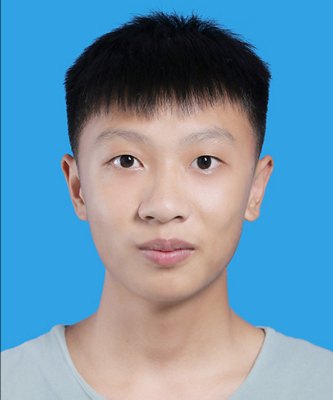
\includegraphics[width=2.2cm,height=2.8cm,keepaspectratio]{assets/avatar.jpg}
\end{minipage}
\vspace{0.8ex}

\section{教育背景}
\datedsubsection{\textbf{广东工业大学}, 能源与动力工程, \textit{本科}}{2022.09 -- 2026.06}
\ \textbf{GPA：3.64 / 5.0}，\textbf{专业排名：前 5\%}，CET-4：550，CET-6：449

\section{科研与项目经历}
\datedsubsection{\textbf{95 kW 水冷式冷凝器设计}，换热器课程设计}{}
\begin{itemize}[parsep=0.1ex]
  \item 面向冷库制冷系统冷凝换热需求，设计采用\textbf{ R22 制冷剂}的\textbf{ 95 kW 水冷式冷凝器}，满足 40 ℃ 冷凝温度与 32 ℃ / 36 ℃ 冷却水进出口工况。
  \item 基于制冷剂状态参数完成\textbf{传热计算、流动阻力计算、结构设计及零部件选型校核}，使用 \textbf{Excel / REFPROP} 处理工质参数并完成装配图与管板零件图设计。
  \item 确定\textbf{ 4 流程、196 根换热管}的管壳式结构方案，设计换热面积约\textbf{ 13.7 m\textsuperscript{2}}，传热面积裕量约\textbf{ 3.8\%}。
\end{itemize}

\datedsubsection{\textbf{HFE-7100/水不互溶混合工质池沸腾传热特性研究}，本科毕业论文}{}
\begin{itemize}[parsep=0.1ex]
  \item 针对\textbf{电子设备低温相变散热}场景，研究\textbf{ HFE-7100/水不互溶混合工质}在光滑铜面与微纳复合结构表面上的\textbf{池沸腾换热性能}。
  \item 基于\textbf{ Kawanami 模型}分析\textbf{ BRT（沸腾工质转换）}与重相液层厚度关系，对 1 mm、3 mm、5 mm 工况进行对比并分析结构失效机理。
  \item 研究结果表明微纳结构未实现持续强化：3 mm 工况下微纳复合表面\textbf{ CHF 为 8.4 W/cm\textsuperscript{2}}，低于光滑铜面\textbf{ 50.2 W/cm\textsuperscript{2}}；最大测量偏差分别为\textbf{ 5.7\%、7.2\%、5.9\%}。
\end{itemize}

\section{专业技能}
\begin{itemize}[parsep=0.1ex]
  \item \textbf{数据处理与可视化：}熟练使用 Python、Pandas、Matplotlib 进行数据处理与可视化
  \item \textbf{机器学习与统计：}熟练使用 scikit-learn、PyTorch；熟悉 SPSS 统计分析操作
  \item \textbf{工程及办公软件：}了解 AutoCAD、SolidWorks 基础操作；熟练使用 Word、Excel、PowerPoint
\end{itemize}

\section{奖学金与荣誉}
\begin{itemize}[parsep=0.1ex]
  \item \textbf{SCI 四区论文}《机器学习辅助的大学生个体碳排放研究：以中国南方地区为例》，第四作者
  \item 2023--2024 学年 ``美的奖学金'' \textbf{一等奖}
  \item 2022--2023、2023--2024 学年年度学习标兵奖学金、年度优秀学生二等奖学金
\end{itemize}

\section{竞赛获奖}
\begin{tabularx}{\textwidth}{@{}Xr@{}}
2023 睿抗机器人开发者大赛（RAICOM）任务应用赛 & \textbf{国赛三等奖} \\
第十五届大学生数学竞赛（非数学 A 类） & \textbf{省赛一等奖} \\
第十五届蓝桥杯全国软件和信息技术专业人才大赛 Python 程序设计大学 B 组 & \textbf{省赛二等奖} \\
2024 年大学生数学建模竞赛 & \textbf{省赛二等奖} \\
2024 睿抗机器人开发者大赛（RAICOM）广东省任务应用赛 & \textbf{省赛三等奖} \\
2023 年 ``深圳杯'' 数学建模挑战赛 & \textbf{省赛三等奖} \\
\end{tabularx}

\section{校园与组织经历}
\datedsubsection{\textbf{广东工业大学计算机学院数智工作室深度学习组组长}}{大二一学年}
\begin{itemize}[parsep=0.1ex]
  \item 负责招新面试、宣讲会介绍、新成员培训与代码指导；带领成员参赛，取得\textbf{数学建模省赛二等奖、RAICOM 省赛二等奖}。
\end{itemize}
\datedsubsection{\textbf{学院心理社团宣传部部长}}{大二一学年}
\begin{itemize}[parsep=0.1ex]
  \item 负责活动推文撰写审核及心理主题活动组织协调，推进宣传任务分工与现场协作。
\end{itemize}

\end{document}
